\section{Implementacja systemu RiskScoop AI}
\label{chap:implementacja}

Rozdział przedstawia szczegóły implementacji systemu RiskScoop AI. Pełny kod źródłowy znajduje się w~załączniku~A.

\subsection{Implementacja backendu}

\subsubsection{Konfiguracja AgentOS}

Agent został zaimplementowany z~wykorzystaniem frameworka Agno AgentOS. Konfiguracja agenta obejmuje:

\begin{itemize}
    \item definicję modelu LLM (Google Gemini 3 Pro),
    \item rejestrację 6 narzędzi z~dekoratorem \texttt{@tool},
    \item konfigurację persystencji sesji (SQLite),
    \item instrukcje systemowe ze schematami danych,
    \item parametry historii konwersacji (5 ostatnich odpowiedzi).
\end{itemize}

AgentOS automatycznie generuje aplikację FastAPI z~endpointami REST do komunikacji z~agentem, persystencji sesji oraz zarządzania historią konwersacji.

\subsubsection{Implementacja narzędzia get\_division}

Narzędzie pobiera granice administracyjne w~dwóch krokach:

\textbf{Krok 1 -- Wyszukanie lokalizacji (Nominatim API):}
\begin{itemize}
    \item zapytanie do \texttt{nominatim.openstreetmap.org/search},
    \item parametry: \texttt{q=nazwa}, \texttt{format=json}, \texttt{polygon\_geojson=1},
    \item odpowiedź zawiera \texttt{osm\_id} oraz podstawową geometrię.
\end{itemize}

\textbf{Krok 2 -- Pobranie szczegółowej geometrii (Overpass API):}
\begin{itemize}
    \item zapytanie OverpassQL dla relacji z~\texttt{osm\_id},
    \item odpowiedź zawiera listę segmentów (ways) tworzących granicę.
\end{itemize}

\subsubsection{Algorytm assemble\_rings}

OpenStreetMap przechowuje granice administracyjne jako oddzielne segmenty (ways), które muszą zostać połączone w~zamknięte pierścienie. Algorytm \texttt{assemble\_rings} realizuje to zadanie:

\textbf{Dane wejściowe:} Lista segmentów, każdy jako tablica współrzędnych $[(x_1, y_1), (x_2, y_2), ...]$

\begin{samepage}
\textbf{Algorytm:}
\begin{enumerate}
    \item inicjalizacja: weź pierwszy segment jako początek pierścienia,
    \item dla każdego pozostałego segmentu:
    \begin{itemize}
        \item porównaj punkt końcowy pierścienia z~punktami segmentu,
        \item jeśli pasuje początek segmentu -- dołącz segment,
        \item jeśli pasuje koniec segmentu -- odwróć i~dołącz,
        \item jeśli pasuje do początku pierścienia -- dołącz na początek,
    \end{itemize}
    \item powtarzaj aż wszystkie segmenty zostaną połączone,
    \item jeśli pierścień nie jest zamknięty -- dodaj pierwszy punkt na koniec.
\end{enumerate}
\end{samepage}

\textbf{Złożoność:} $O(n^2)$ gdzie $n$ to liczba segmentów. Dla typowych granic ($n < 100$) czas wykonania $< 10$~ms.

\subsubsection{Implementacja narzędzia get\_overture\_data}

Narzędzie komunikuje się z~dedykowanym API Overture Maps:

\textbf{Parametry zapytania:}
\begin{itemize}
    \item \texttt{bbox} -- bounding box z~warstwy AOI $[min\_lon, min\_lat, max\_lon, max\_lat]$,
    \item \texttt{category} -- kategoria obiektów (healthcare, education, etc.).
\end{itemize}

\textbf{Odpowiedź:} GeoJSON FeatureCollection z~obiektami zawierającymi:
\begin{itemize}
    \item \texttt{geometry} -- punkt lub wielokąt,
    \item \texttt{properties.name} -- nazwa obiektu,
    \item \texttt{properties.category} -- kategoria,
    \item \texttt{properties.confidence} -- pewność klasyfikacji.
\end{itemize}

\subsubsection{Implementacja narzędzia get\_flood\_forecast}

Narzędzie pobiera dane z~Copernicus Climate Data Store (CDS) i~konwertuje raster na punkty:

\textbf{Pobieranie danych:}
\begin{itemize}
    \item API: \texttt{cds.climate.copernicus.eu},
    \item dataset: \texttt{cems-glofas-forecast},
    \item format: GeoTIFF z~klasami głębokości (1--5),
    \item przycinanie do bounding box AOI.
\end{itemize}

\textbf{Konwersja raster $\rightarrow$ punkty:}
\begin{enumerate}
    \item iteracja po pikselach rastra,
    \item dla każdego piksela z~wartością 1--5:
    \begin{itemize}
        \item oblicz współrzędne środka piksela,
        \item utwórz punkt GeoJSON,
        \item przypisz atrybuty: \texttt{flood\_depth\_class}, \texttt{risk\_level},
    \end{itemize}
    \item zwróć GeoDataFrame z~punktami.
\end{enumerate}

\textbf{Mapowanie klas na ryzyko:}
\begin{itemize}
    \item klasa 1 (0--0.5m) $\rightarrow$ \texttt{risk\_level = "low"},
    \item klasa 2 (0.5--1m) $\rightarrow$ \texttt{risk\_level = "medium"},
    \item klasy 3--5 (>1m) $\rightarrow$ \texttt{risk\_level = "high"}.
\end{itemize}

\subsubsection{Implementacja narzędzia intersect\_flood\_zones}

Narzędzie wykonuje analizę przestrzenną z~wykorzystaniem biblioteki GeoPandas:

\textbf{Algorytm:}
\begin{enumerate}
    \item wczytaj warstwę obiektów i~warstwę powodziową,
    \item buforuj obiekty o~zadaną odległość (domyślnie 100~m):
    \begin{itemize}
        \item przelicz stopnie na metry: $buffer\_deg = buffer\_m / 111320$,
        \item zastosuj \texttt{geometry.buffer(buffer\_deg)},
    \end{itemize}
    \item wykonaj spatial join:
    \begin{itemize}
        \item \texttt{gpd.sjoin(features, flood, predicate='intersects')},
    \end{itemize}
    \item agreguj maksymalny poziom ryzyka dla każdego obiektu:
    \begin{itemize}
        \item grupuj po indeksie obiektu,
        \item wybierz \texttt{max(risk\_level)} według kolejności: low < medium < high,
    \end{itemize}
    \item zapisz wynik jako nową warstwę GeoJSON.
\end{enumerate}

\subsection{Implementacja serwisów}

\subsubsection{LayerService}

Serwis zarządza warstwami GeoJSON w~sesji użytkownika:

\begin{itemize}
    \item \textbf{save\_layer(gdf, session, name)} -- zapisuje GeoDataFrame jako plik GeoJSON z~UUID, dodaje referencję do sesji,
    \item \textbf{load\_layer(uuid)} -- wczytuje warstwę z~pliku do GeoDataFrame,
    \item \textbf{list\_layers(session)} -- zwraca listę warstw w~sesji,
    \item \textbf{delete\_layer(uuid)} -- usuwa warstwę z~dysku i~sesji.
\end{itemize}

Warstwy są przechowywane w~katalogu \texttt{output/layers/\{uuid\}.geojson}.

\subsubsection{NominatimService}

Serwis obsługuje komunikację z~API Nominatim i~Overpass:

\begin{itemize}
    \item \textbf{search(query)} -- wyszukiwanie lokalizacji,
    \item \textbf{get\_boundary(osm\_id)} -- pobranie geometrii granicy,
    \item \textbf{assemble\_rings(ways)} -- składanie wielokątów.
\end{itemize}

Serwis implementuje cache wyników (TTL: 1 godzina) oraz rate limiting (1 req/s) zgodnie z~polityką Nominatim.

\subsubsection{GloFASService}

Serwis pobiera i~przetwarza dane powodziowe:

\begin{itemize}
    \item \textbf{get\_forecast(bbox, return\_period)} -- pobranie rastra GloFAS,
    \item \textbf{raster\_to\_points(raster\_path)} -- konwersja na punkty,
    \item \textbf{classify\_risk(depth\_class)} -- mapowanie klasy na poziom ryzyka.
\end{itemize}

\subsection{Implementacja frontendu}

\subsubsection{Architektura komponentów}

Frontend został zaimplementowany jako aplikacja jednostronicowa (Single File Application) w~czystym JavaScript z~następującymi modułami:

\begin{itemize}
    \item \textbf{App} -- główny komponent, zarządzanie stanem aplikacji,
    \item \textbf{ChatPanel} -- wprowadzanie zapytań, wyświetlanie odpowiedzi,
    \item \textbf{MapView} -- mapa Mapbox GL JS z~warstwami,
    \item \textbf{LayerPanel} -- lista warstw, przełączanie widoczności,
    \item \textbf{FeaturePopup} -- szczegóły wybranego obiektu.
\end{itemize}

\subsubsection{Komunikacja z~backendem}

Frontend komunikuje się z~AgentOS przez REST API:

\begin{enumerate}
    \item użytkownik wprowadza zapytanie w~ChatPanel,
    \item zapytanie wysyłane do \texttt{POST /agents/riskscoop-ai/runs},
    \item backend zwraca odpowiedź agenta oraz listę utworzonych warstw,
    \item frontend pobiera warstwy z~\texttt{GET /layers/\{uuid\}},
    \item MapView renderuje warstwy na mapie.
\end{enumerate}

\subsubsection{Wizualizacja warstw}

Warstwy są renderowane z~następującą kolorystyką:

\begin{itemize}
    \item \textbf{AOI (granice)} -- niebieski kontur, przezroczyste wypełnienie,
    \item \textbf{obiekty bez ryzyka} -- szare punkty/wielokąty,
    \item \textbf{ryzyko niskie} -- zielone (\texttt{\#22c55e}),
    \item \textbf{ryzyko średnie} -- pomarańczowe (\texttt{\#f97316}),
    \item \textbf{ryzyko wysokie} -- czerwone (\texttt{\#ef4444}).
\end{itemize}

\subsection{Własne endpointy API}

Oprócz endpointów generowanych przez AgentOS, zdefiniowano własne endpointy:

\begin{itemize}
    \item \texttt{GET /layers/\{uuid\}} -- pobranie warstwy GeoJSON,
    \item \texttt{GET /app-config} -- konfiguracja frontendu (URL mapy, kolory),
    \item \texttt{DELETE /layers/\{uuid\}} -- usunięcie warstwy.
\end{itemize}

\subsection{Przykłady użycia systemu}

Poniżej przedstawiono przykładowe interakcje z~systemem, które posłużą do testów w~rozdziale~\ref{chap:testy}.

\subsubsection{Przykład 1: Szpitale w~Genewie}

\begin{samepage}
\textbf{Zapytanie:} \textit{,,Find hospitals at flood risk in Geneva, Switzerland''}

\textbf{Sekwencja wywołań agenta:}
\begin{enumerate}
    \item \texttt{get\_division("Geneva, Switzerland", "geneva\_aoi")},
    \item \texttt{get\_overture\_data("geneva\_aoi", "healthcare", "geneva\_hospitals")},
    \item \texttt{get\_flood\_forecast("geneva\_aoi", "RP100", "geneva\_flood")},
    \item \texttt{intersect\_flood\_zones("geneva\_hospitals", "geneva\_flood", "hospitals\_at\_risk")}.
\end{enumerate}

\textbf{Oczekiwany wynik:} Lista szpitali z~przypisanym poziomem ryzyka, mapa z~wizualizacją.
\end{samepage}

\begin{figure}[H]
    \centering
    \makebox[\textwidth]{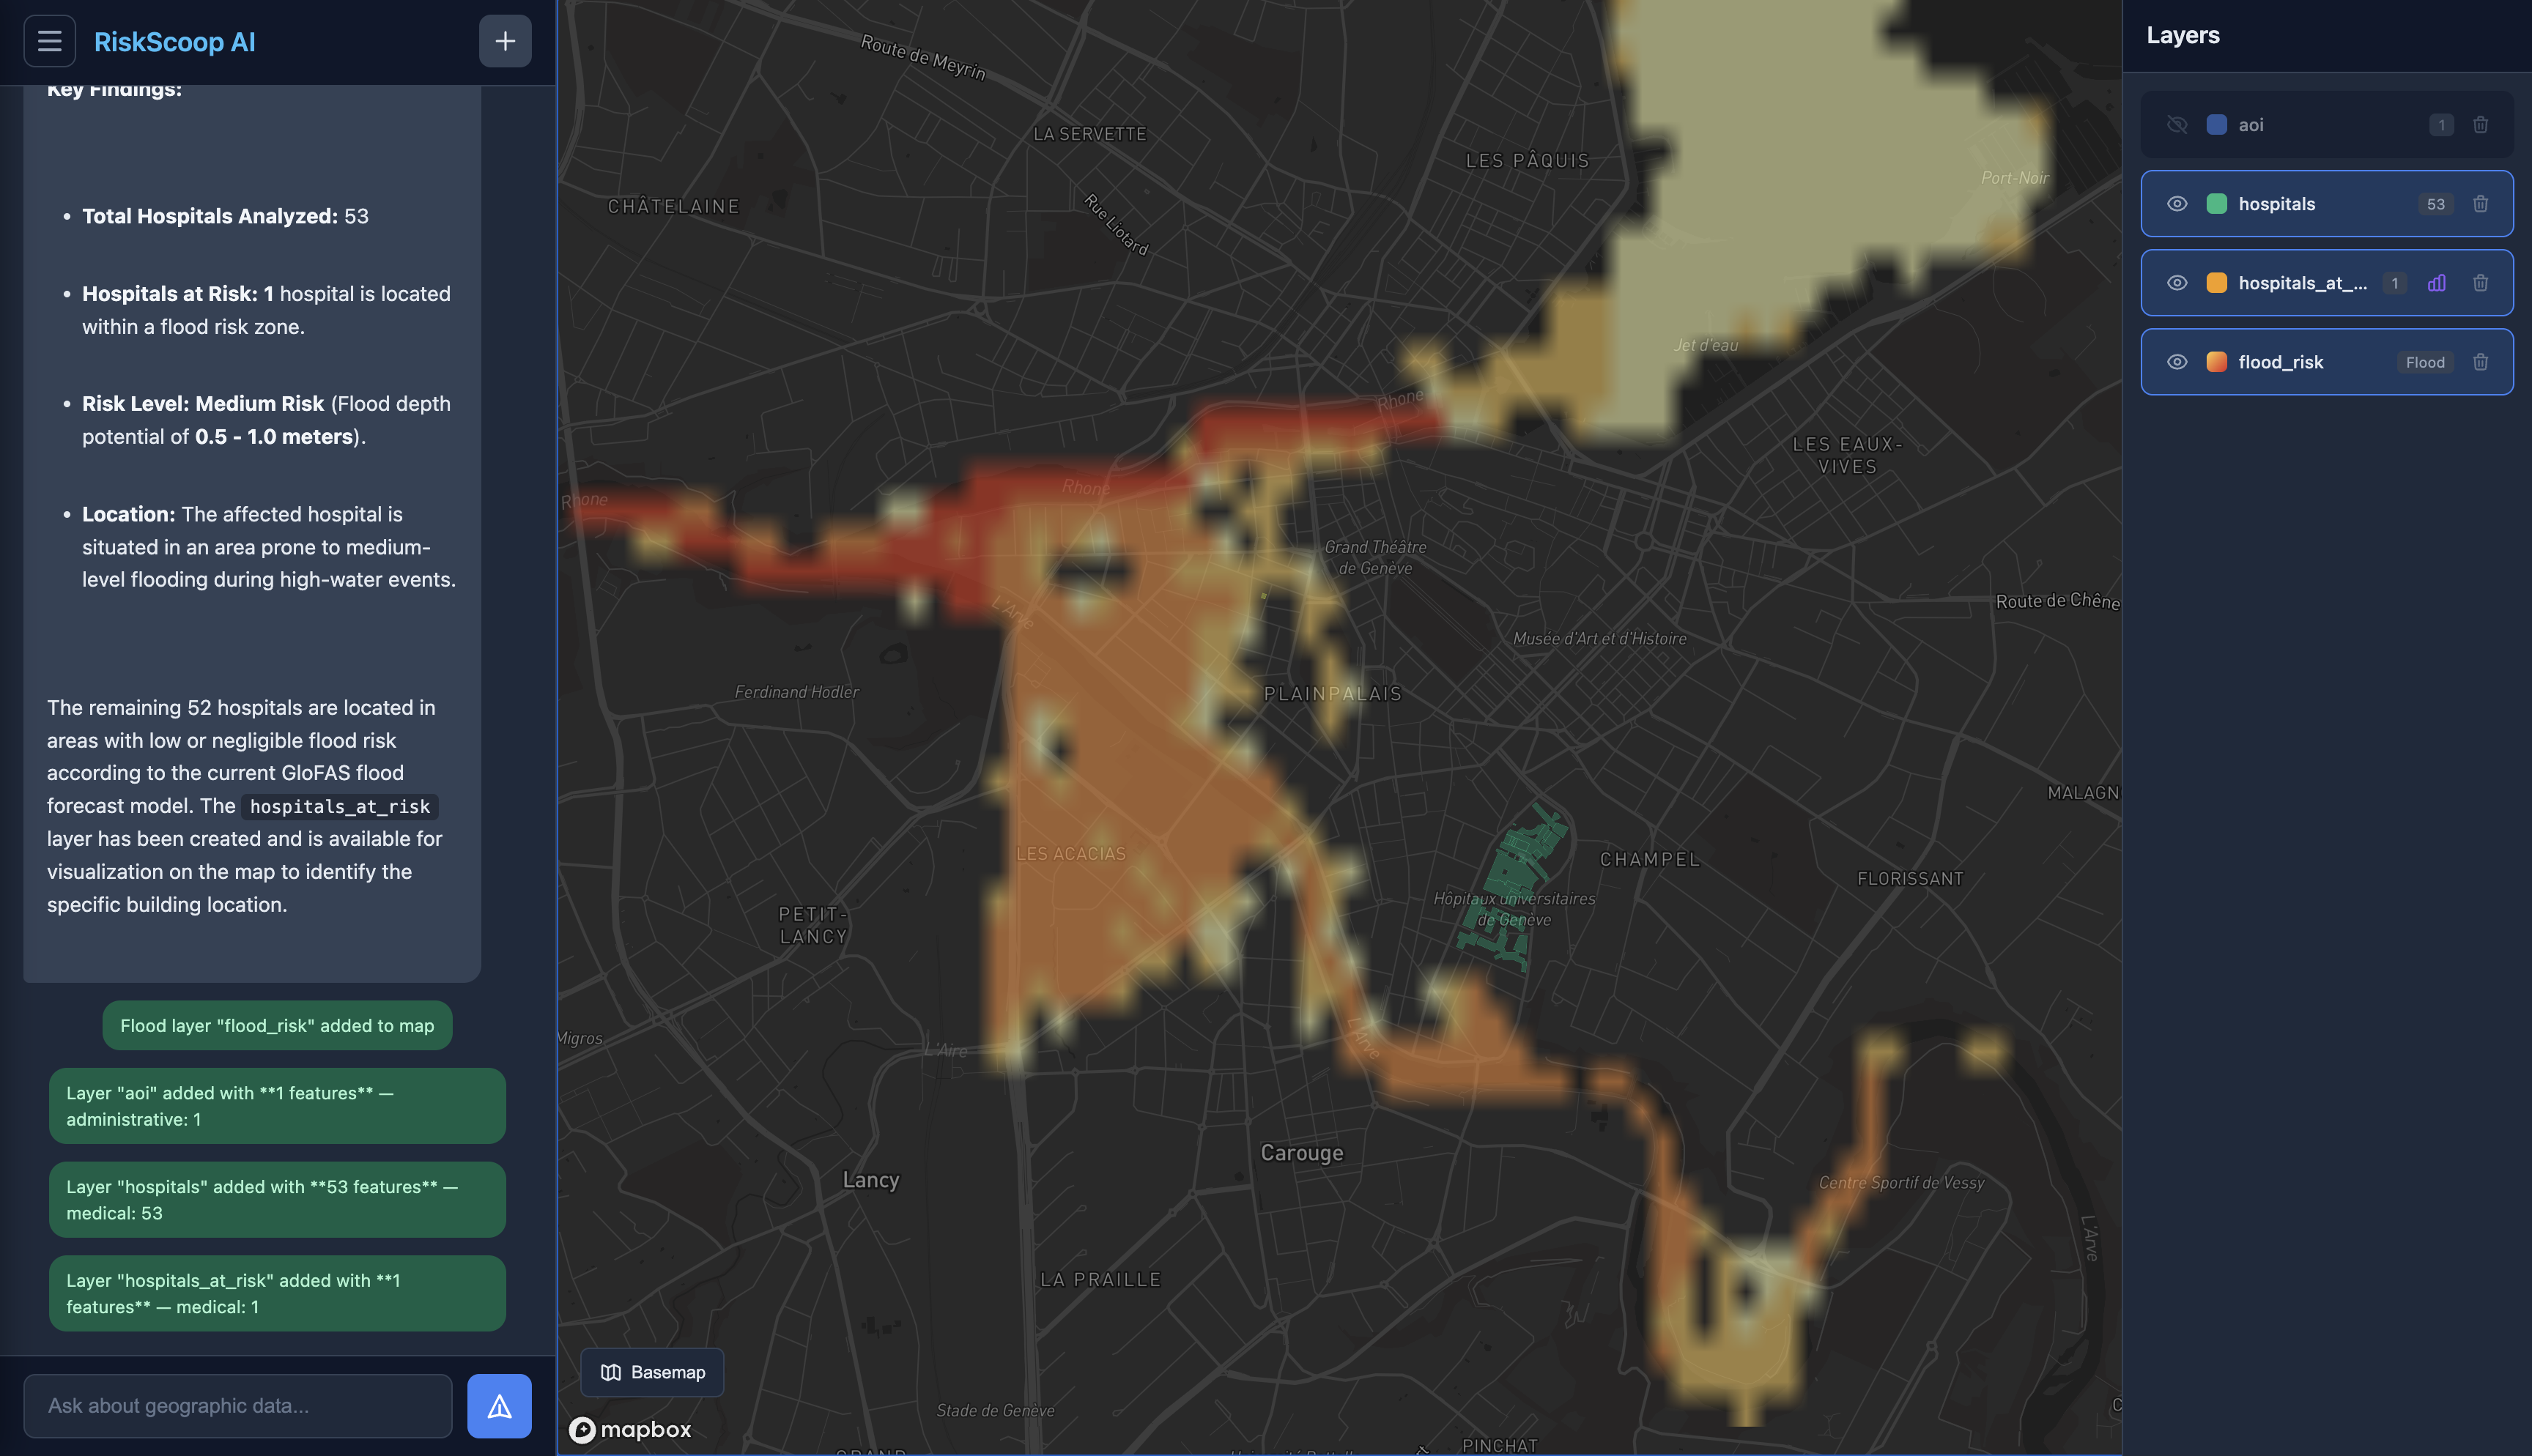
\includegraphics[width=1.15\textwidth]{Figures/Szpitale_w_Genewie.png}}
    \caption{Przykład analizy: szpitale w~Genewie (opracowanie własne)}
    \label{fig:example_geneva}
\end{figure}

\subsubsection{Przykład 2: Szkoły w~Warszawie}

\begin{samepage}
\textbf{Zapytanie:} \textit{,,Which schools in Warsaw are at high flood risk?''}

\textbf{Sekwencja wywołań agenta:}
\begin{enumerate}
    \item \texttt{get\_division("Warsaw, Poland", "warsaw\_aoi")},
    \item \texttt{get\_overture\_data("warsaw\_aoi", "education", "warsaw\_schools")},
    \item \texttt{get\_flood\_forecast("warsaw\_aoi", "RP100", "warsaw\_flood")},
    \item \texttt{intersect\_flood\_zones("warsaw\_schools", "warsaw\_flood", "schools\_at\_risk")}.
\end{enumerate}

\textbf{Oczekiwany wynik:} Lista szkół z~wysokim ryzykiem powodziowym.
\end{samepage}

\begin{figure}[H]
    \centering
    \makebox[\textwidth]{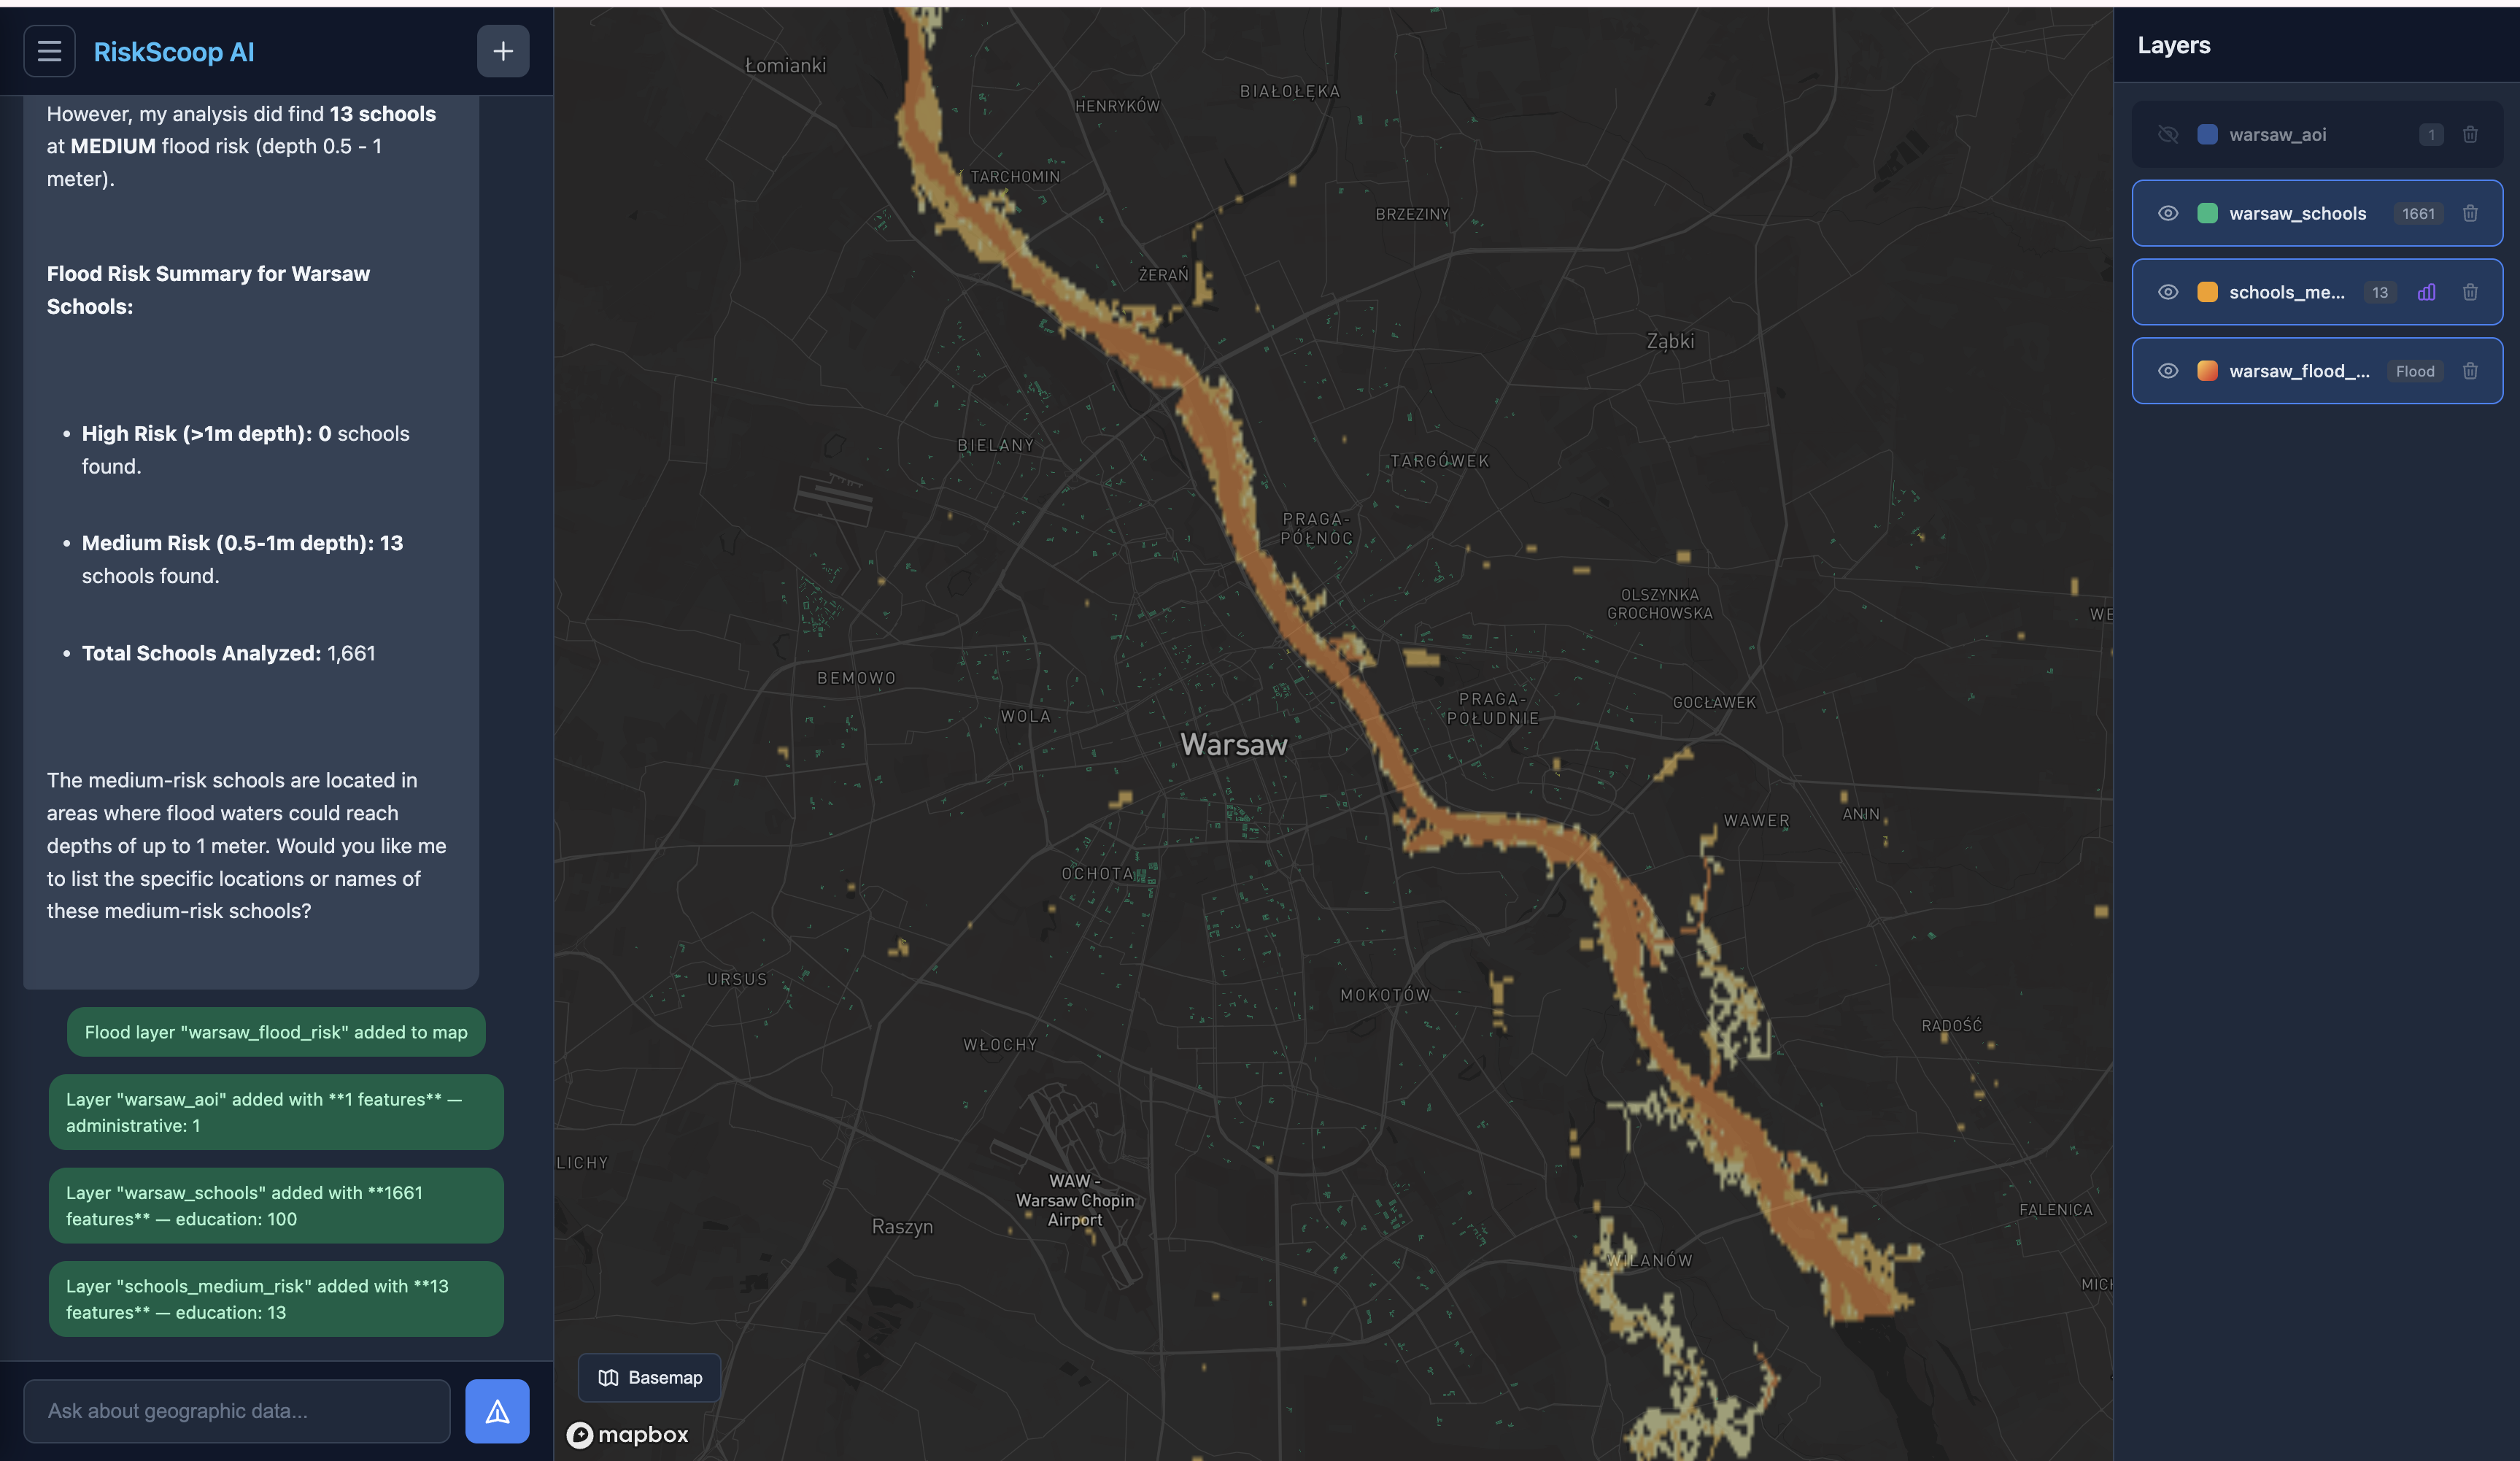
\includegraphics[width=1.15\textwidth]{Figures/Szkoly_w_Warszawie.png}}
    \caption{Przykład analizy: szkoły w~Warszawie (opracowanie własne)}
    \label{fig:example_warsaw}
\end{figure}

\subsubsection{Przykład 3: Budynki w~Krakowie}

\begin{samepage}
\textbf{Zapytanie:} \textit{,,Show all buildings at flood risk in Kraków''}

\textbf{Sekwencja wywołań agenta:}
\begin{enumerate}
    \item \texttt{get\_division("Kraków, Poland", "krakow\_aoi")},
    \item \texttt{get\_overture\_data("krakow\_aoi", "buildings", "krakow\_buildings")},
    \item \texttt{get\_flood\_forecast("krakow\_aoi", "RP50", "krakow\_flood")},
    \item \texttt{intersect\_flood\_zones("krakow\_buildings", "krakow\_flood", "buildings\_at\_risk")}.
\end{enumerate}

\textbf{Oczekiwany wynik:} Mapa budynków zagrożonych powodzią w~Krakowie.
\end{samepage}

\begin{figure}[H]
    \centering
    \makebox[\textwidth]{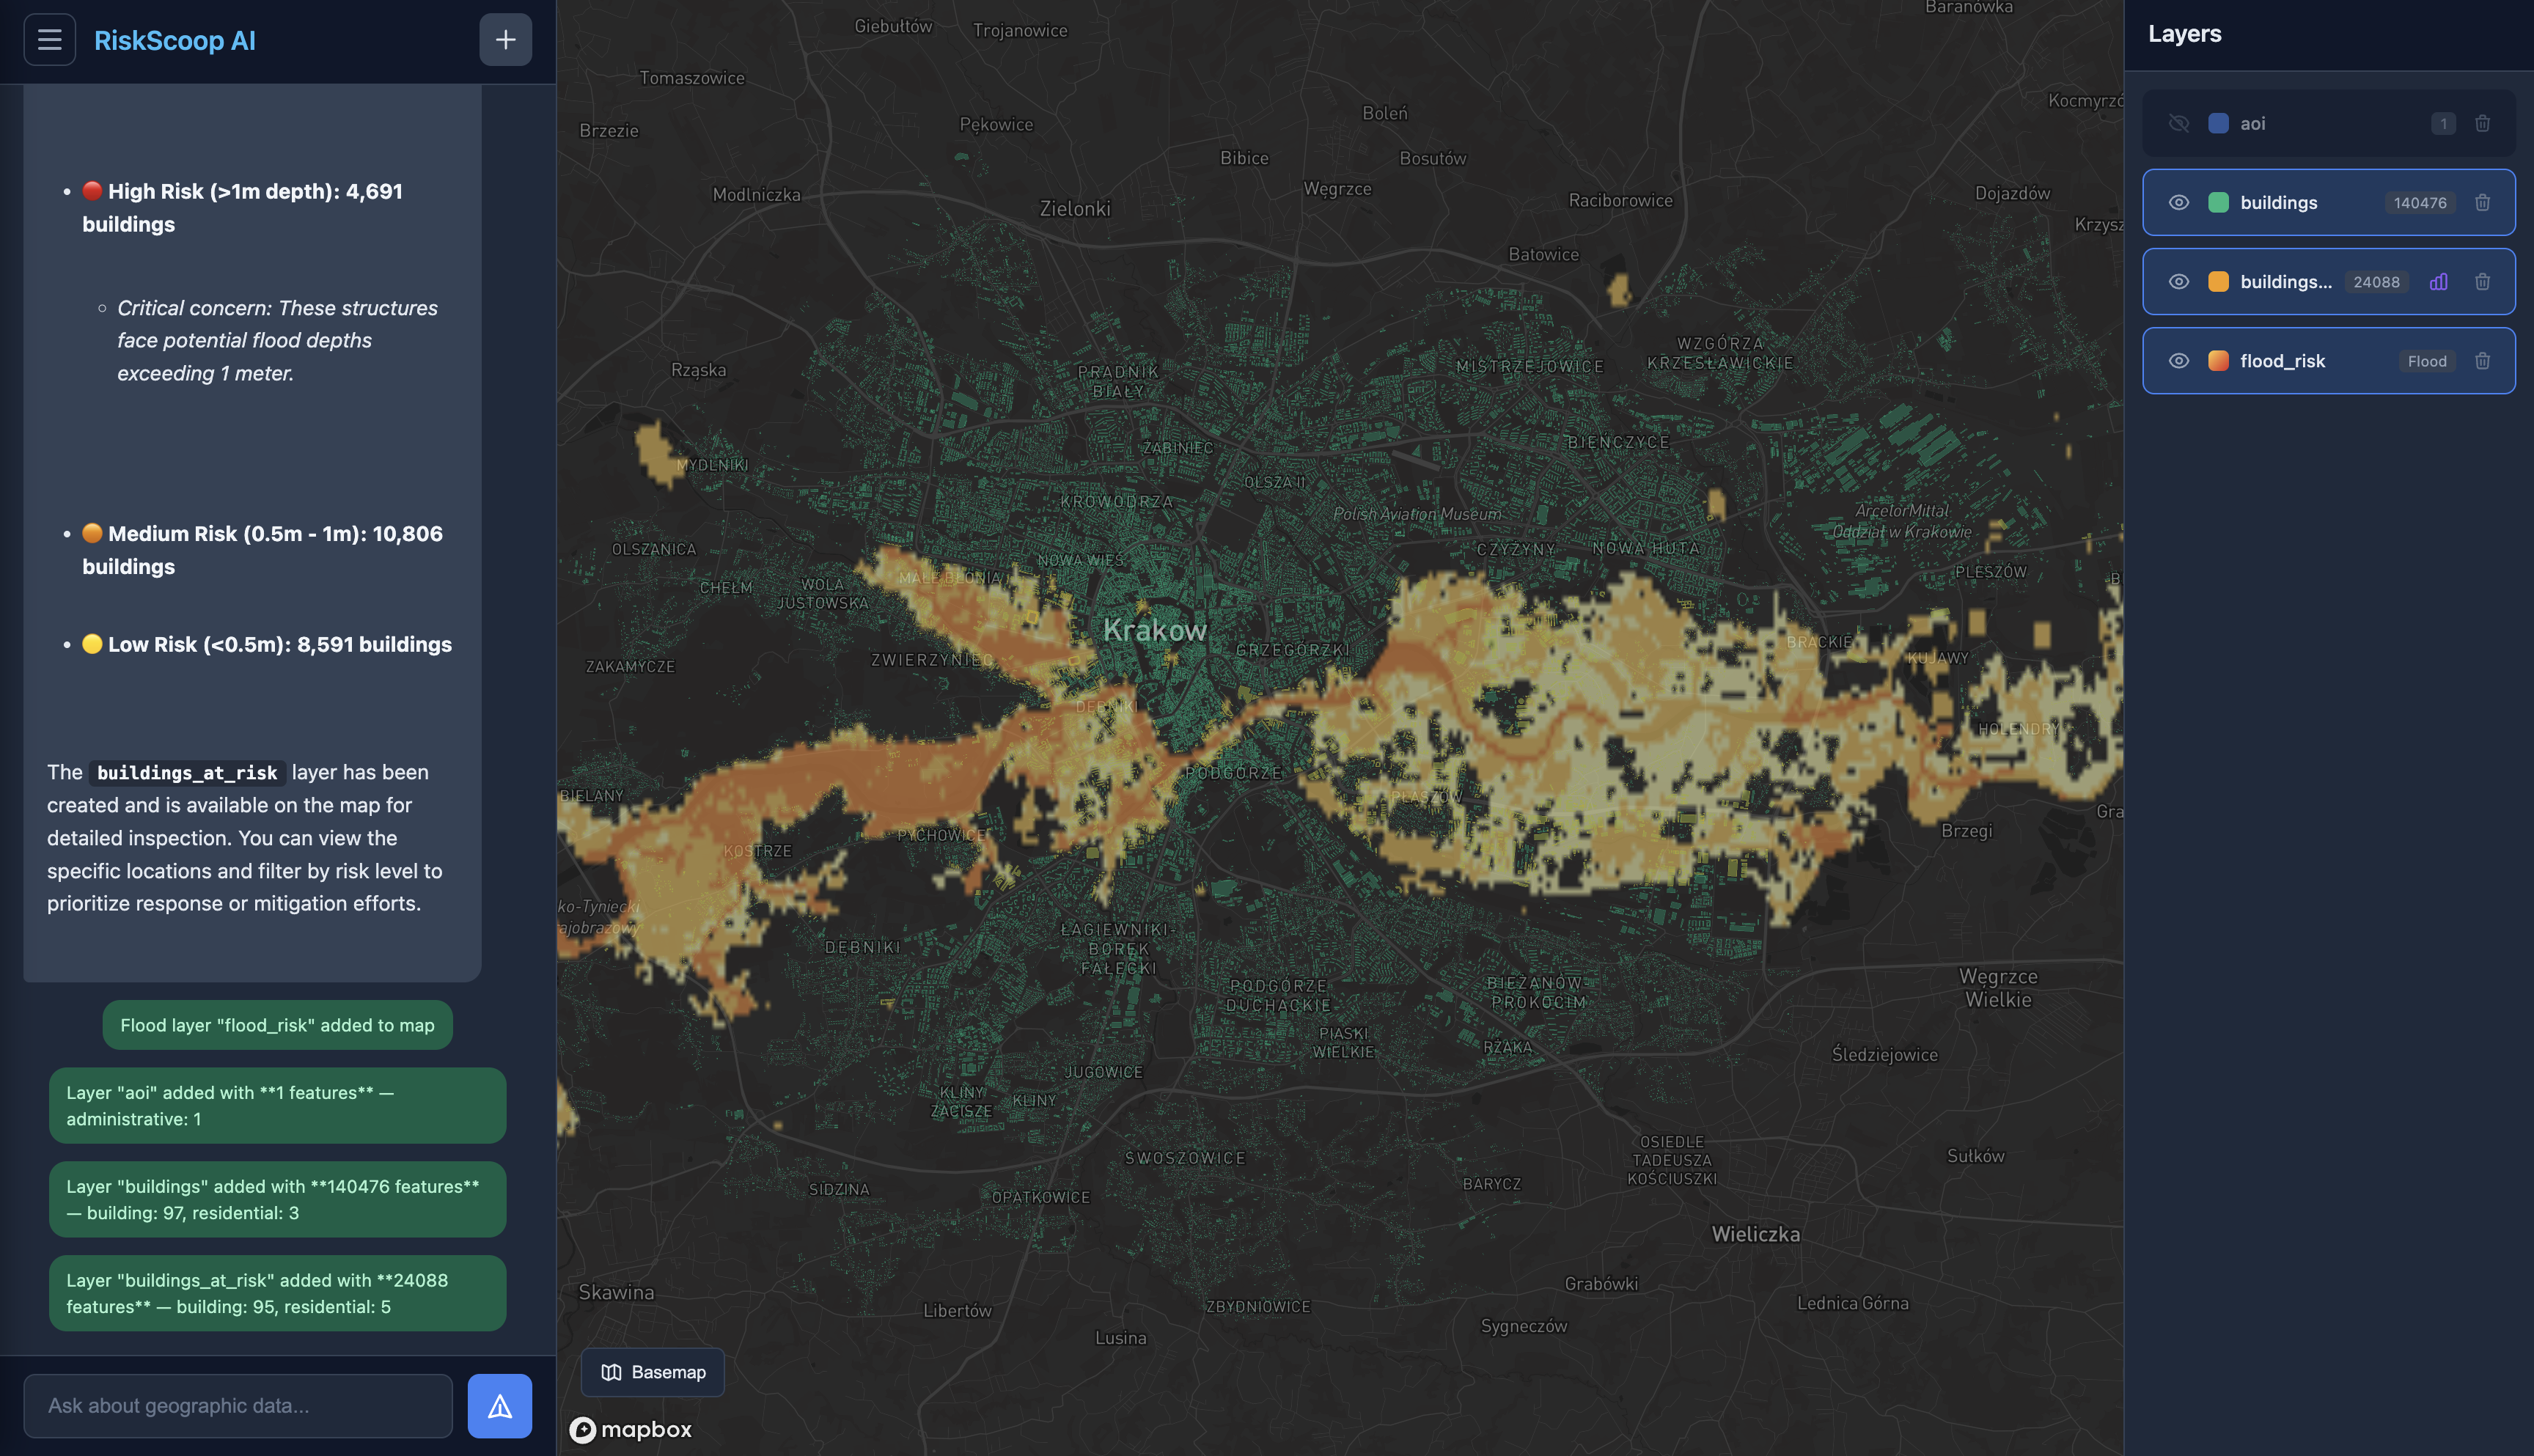
\includegraphics[width=1.15\textwidth]{Figures/Budynki_w_Krakowie.png}}
    \caption{Przykład analizy: budynki w~Krakowie (opracowanie własne)}
    \label{fig:example_krakow}
\end{figure}

\subsubsection{Przykład 4: Infrastruktura w~okolicach Płocka}

\begin{samepage}
\textbf{Zapytanie:} \textit{,,Find critical infrastructure at flood risk in Płock, Poland''}

\textbf{Sekwencja wywołań agenta:}
\begin{enumerate}
    \item \texttt{get\_division("Płock, Poland", "plock\_aoi")},
    \item \texttt{get\_overture\_data("plock\_aoi", "infrastructure", "plock\_infrastructure")},
    \item \texttt{get\_flood\_forecast("plock\_aoi", "RP100", "plock\_flood")},
    \item \texttt{intersect\_flood\_zones("plock\_infrastructure", "plock\_flood", "infrastructure\_at\_risk")}.
\end{enumerate}

\textbf{Oczekiwany wynik:} Mapa infrastruktury zagrożonej powodzią w~Płocku. Okolice Płocka doświadczyły katastrofalnej powodzi w~1981~roku, spowodowanej zatorami lodowymi na Wiśle, która dotknęła Kępę Polską, Dobrzyków oraz dzielnicę Płock-Radziwie.
\end{samepage}

\begin{figure}[H]
    \centering
    \makebox[\textwidth]{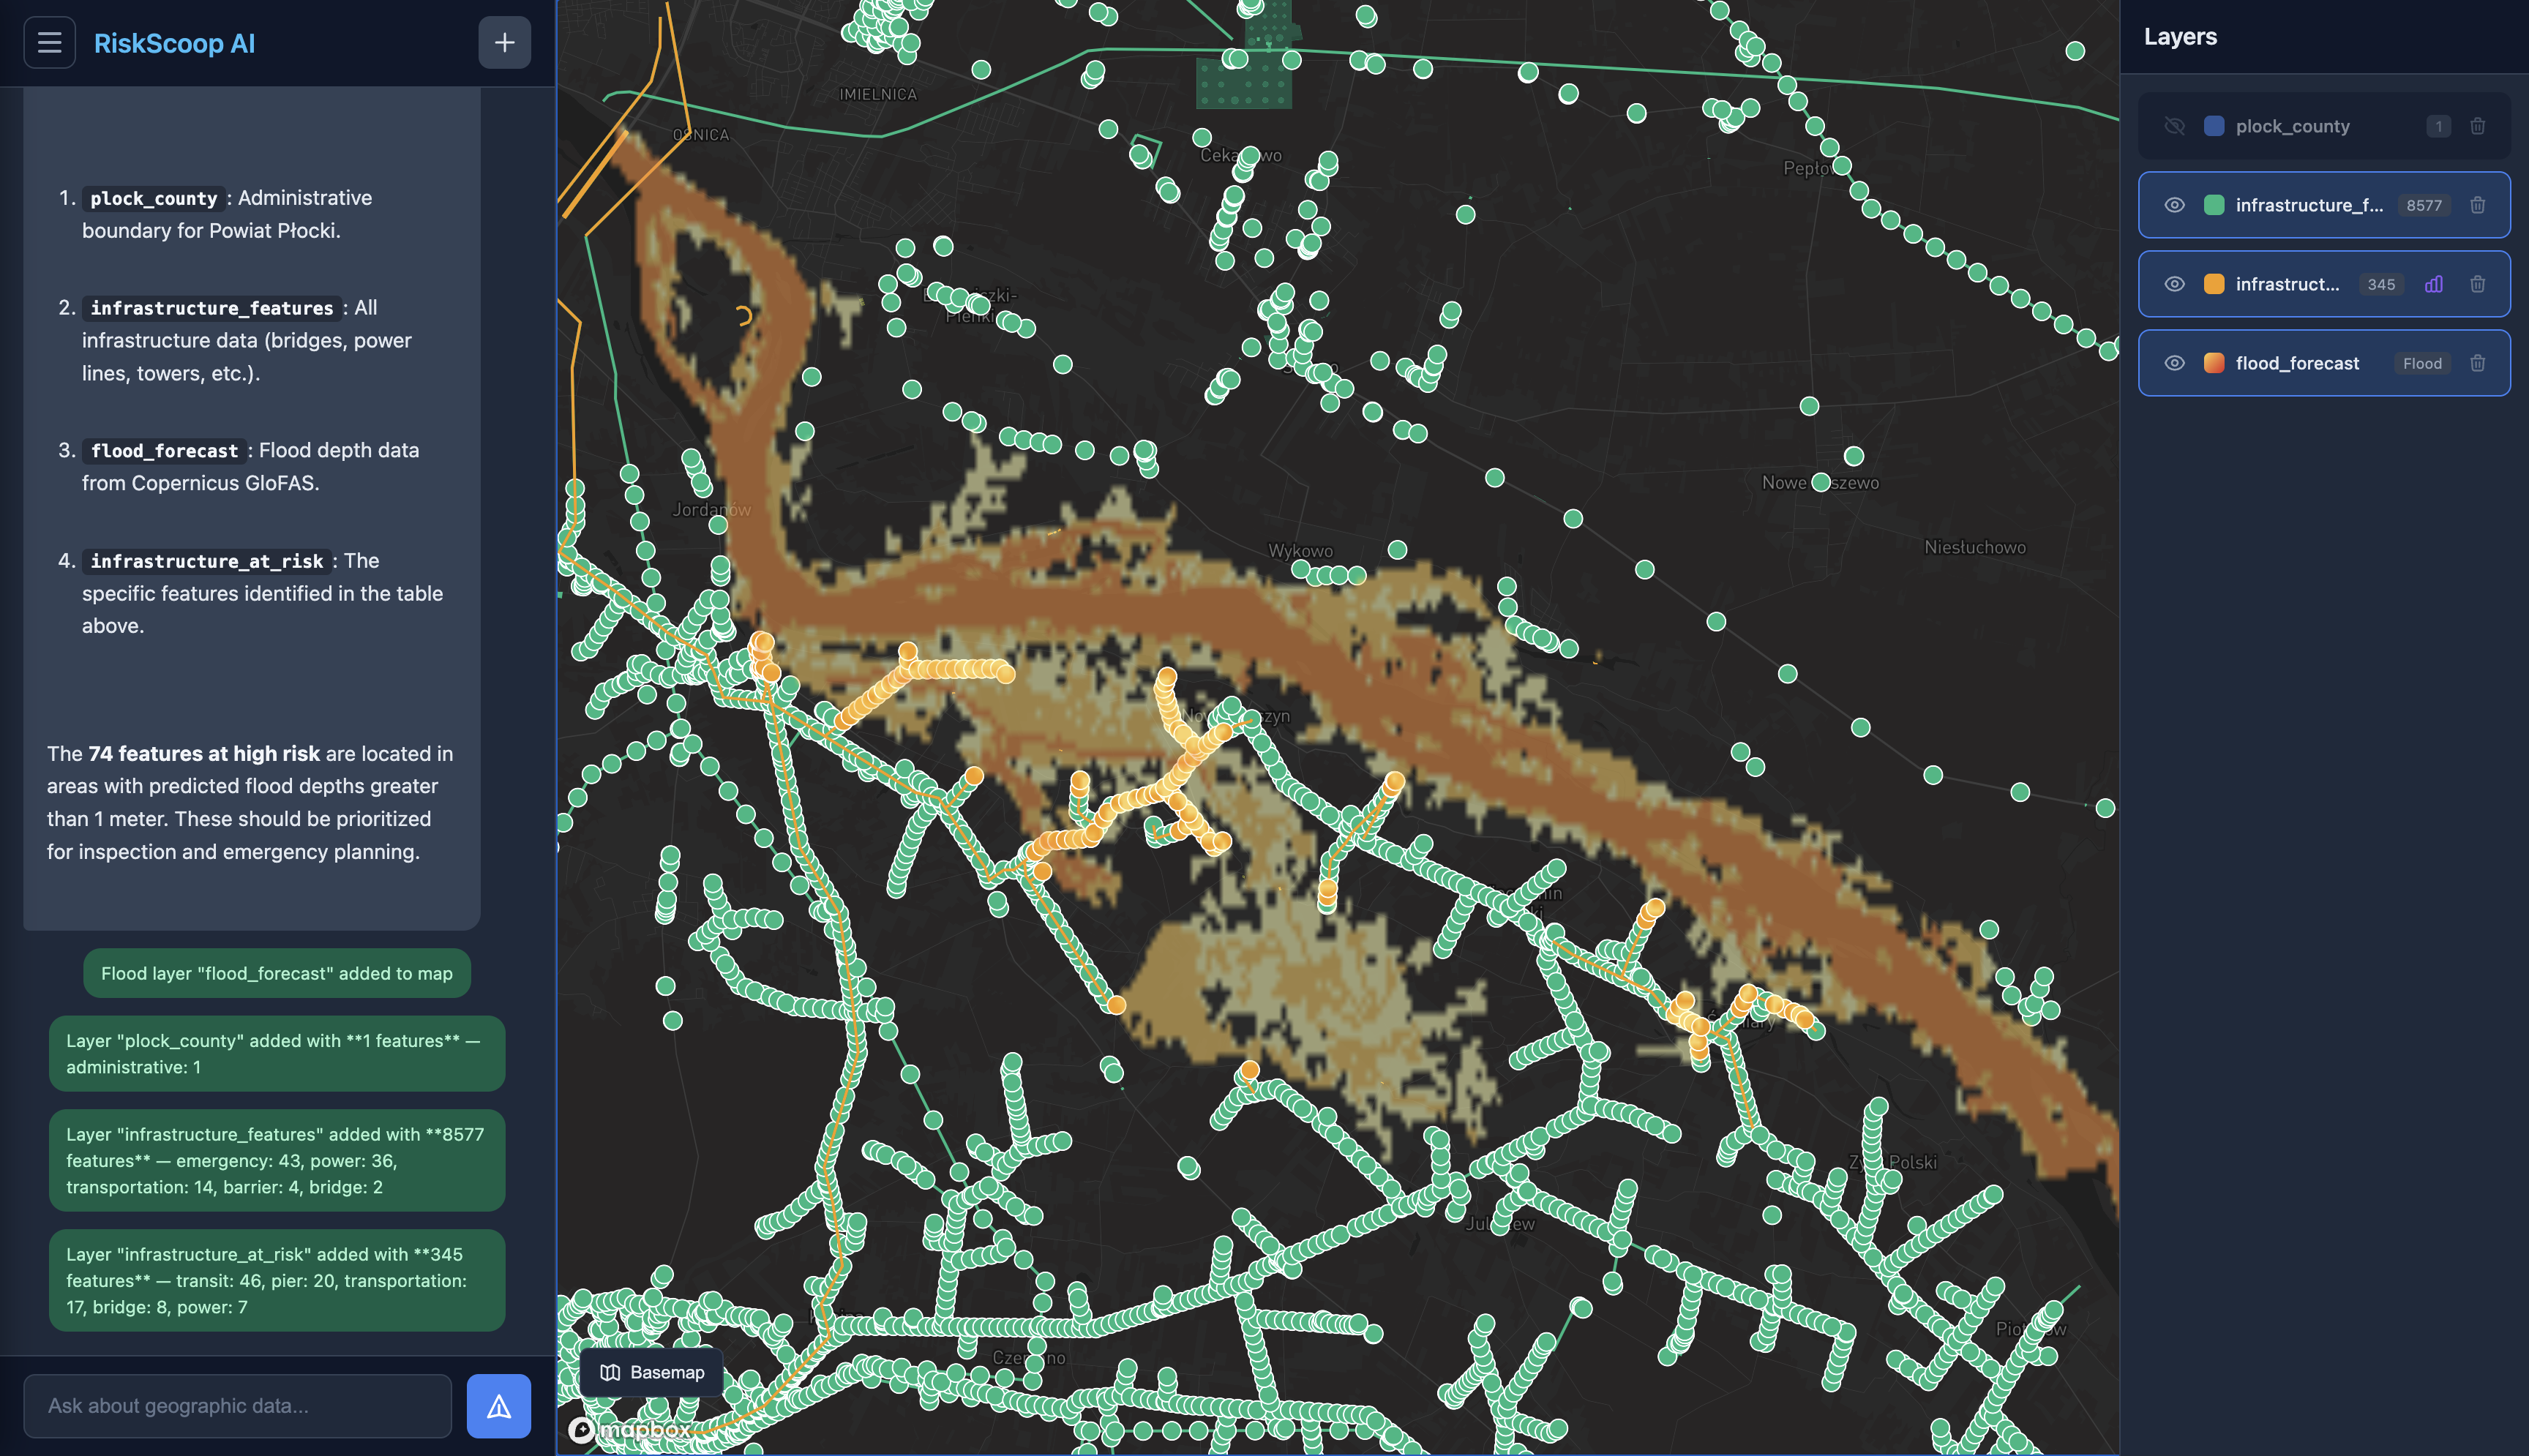
\includegraphics[width=1.15\textwidth]{Figures/Infrastruktura_w_Plocku.png}}
    \caption{Przykład analizy: infrastruktura w~okolicach Płocka (opracowanie własne)}
    \label{fig:example_plock}
\end{figure}

\subsubsection{Przykład 5: Infrastruktura we Wrocławiu}

\begin{samepage}
\textbf{Zapytanie:} \textit{,,Show infrastructure at flood risk in Wrocław, Poland''}

\textbf{Sekwencja wywołań agenta:}
\begin{enumerate}
    \item \texttt{get\_division("Wrocław, Poland", "wroclaw\_aoi")},
    \item \texttt{get\_overture\_data("wroclaw\_aoi", "infrastructure", "wroclaw\_infrastructure")},
    \item \texttt{get\_flood\_forecast("wroclaw\_aoi", "RP100", "wroclaw\_flood")},
    \item \texttt{intersect\_flood\_zones("wroclaw\_infrastructure", "wroclaw\_flood", "infrastructure\_at\_risk")}.
\end{enumerate}

\textbf{Oczekiwany wynik:} Mapa infrastruktury zagrożonej powodzią we Wrocławiu. Wrocław doświadczył Powodzi Tysiąclecia w~1997~roku, która spowodowała katastrofalne zniszczenia w~centrum miasta, na osiedlu Kozanów oraz na terenach zalewowych Odry.
\end{samepage}

\begin{figure}[H]
    \centering
    \makebox[\textwidth]{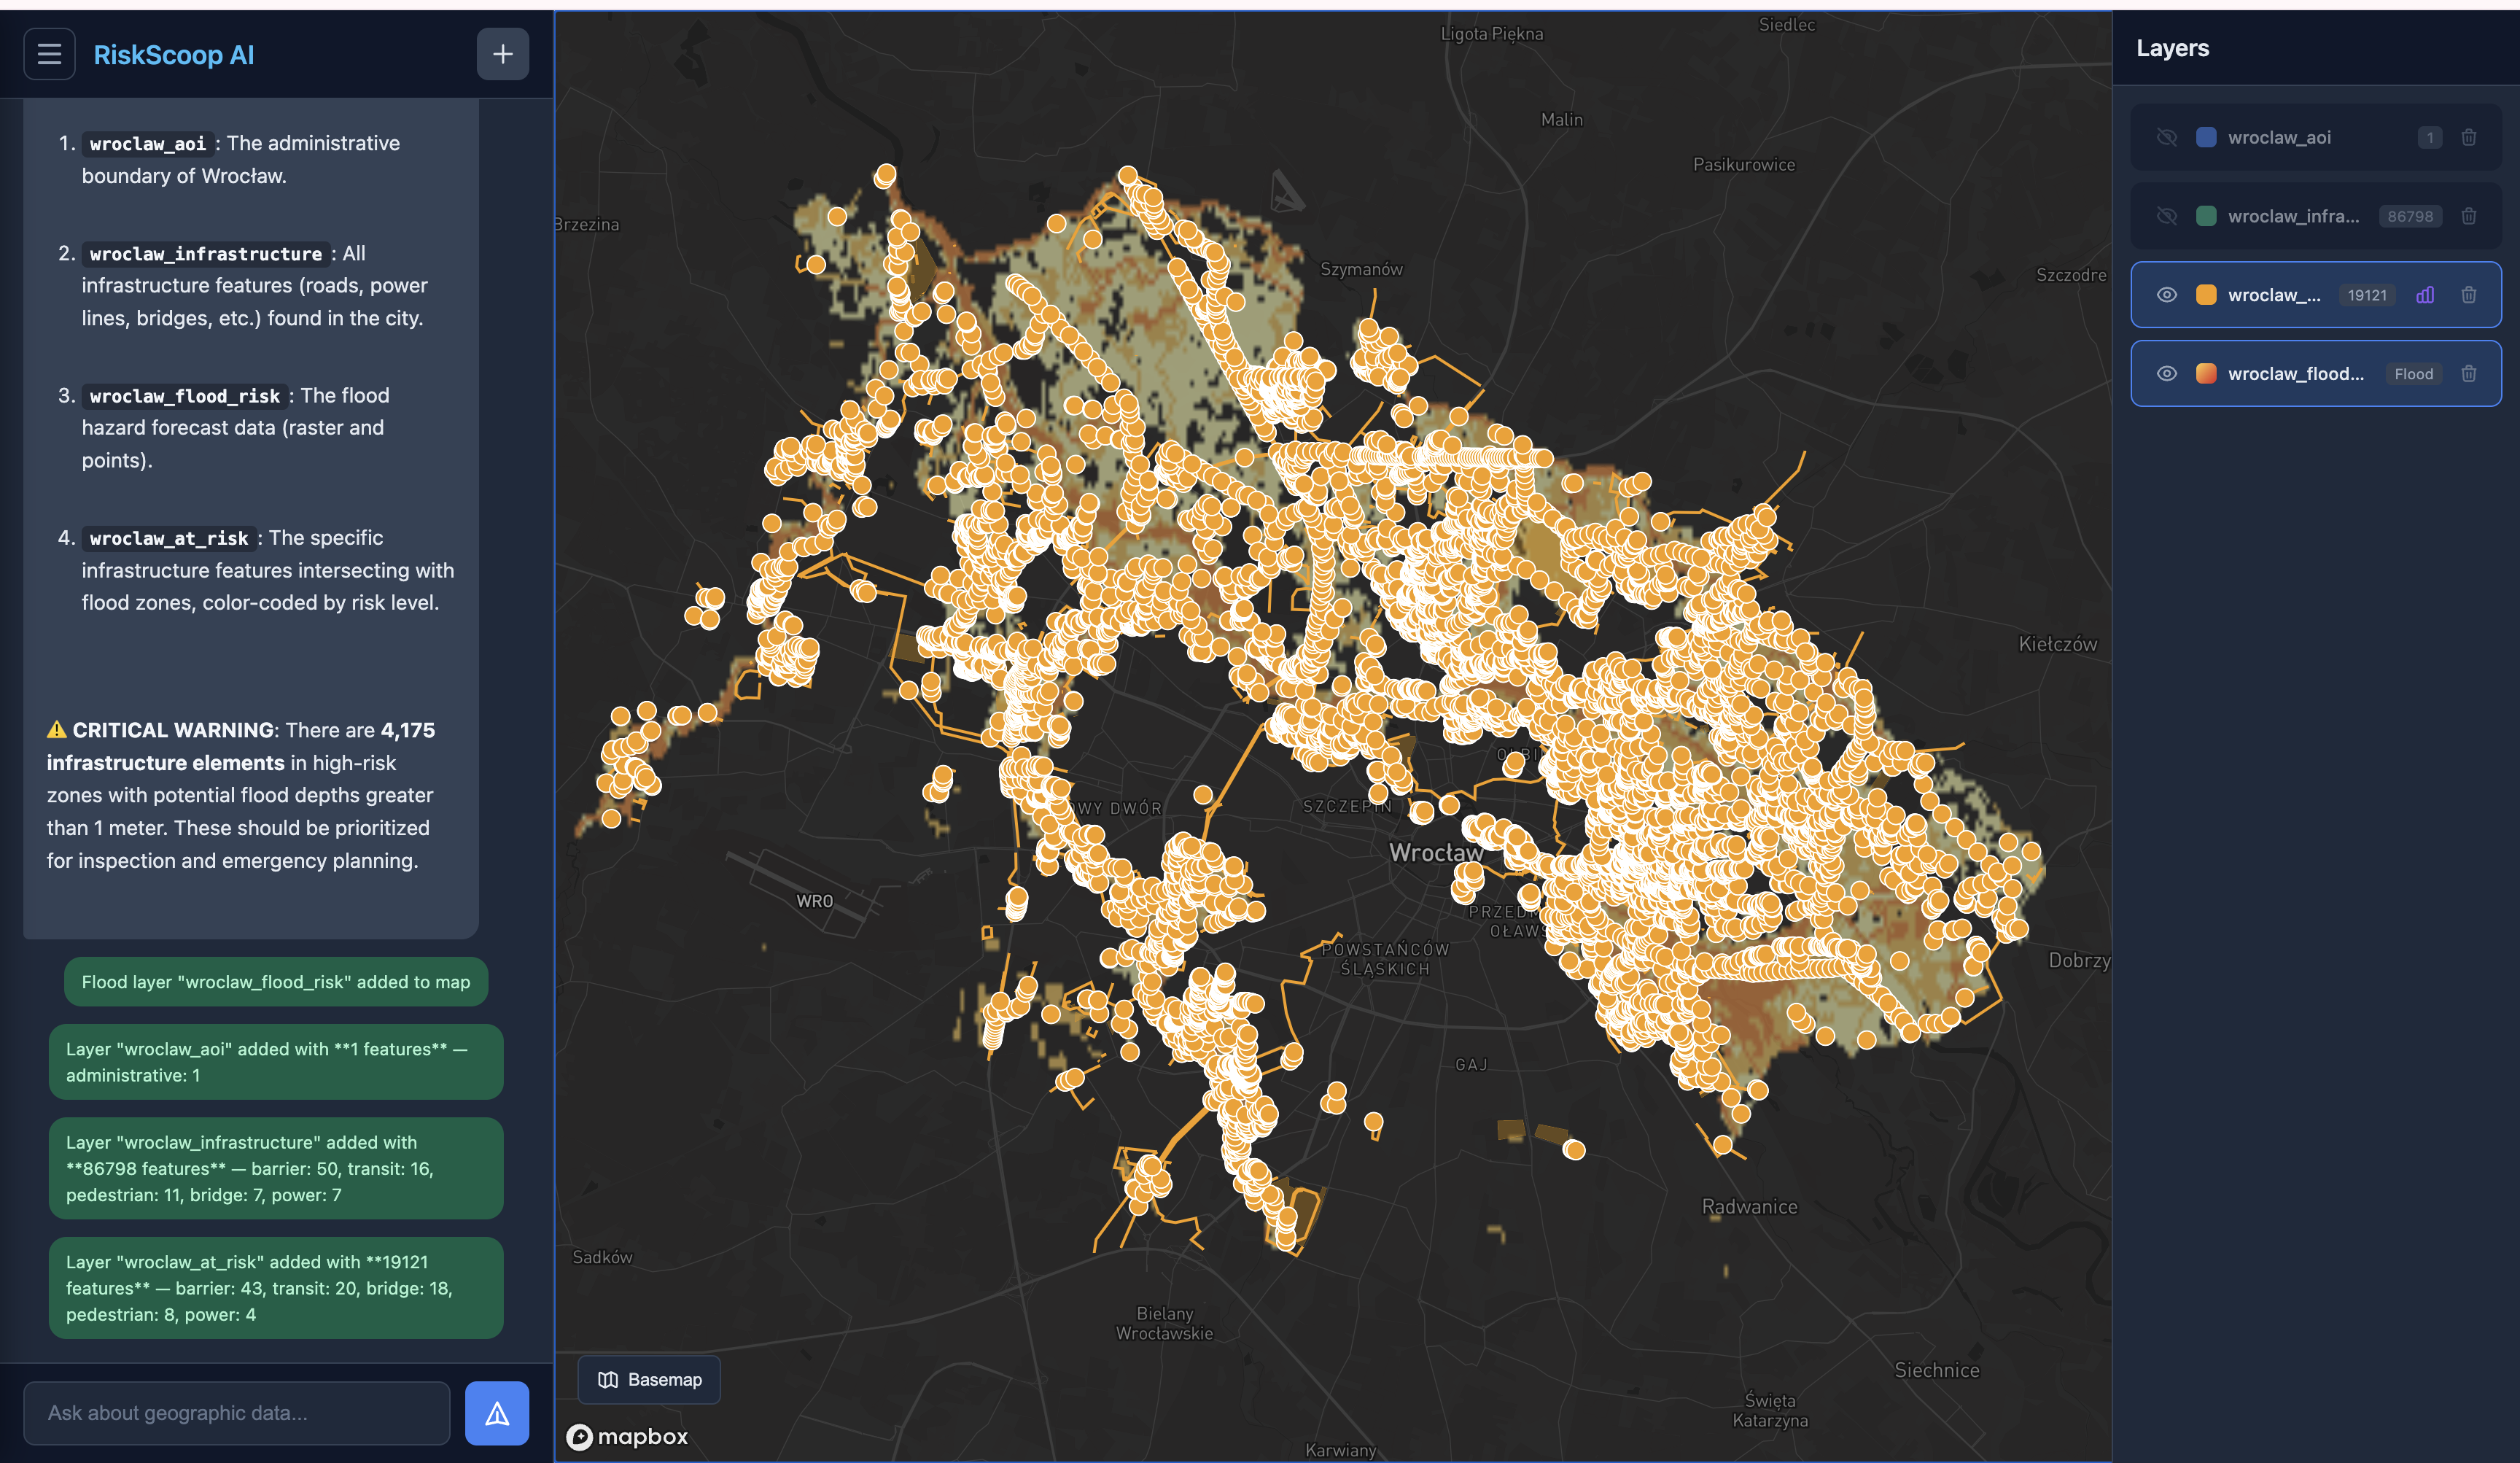
\includegraphics[width=1.15\textwidth]{Figures/Infrastruktura_we_Wroclawiu.png}}
    \caption{Przykład analizy: infrastruktura we Wrocławiu (opracowanie własne)}
    \label{fig:example_wroclaw}
\end{figure}

\subsection{Podsumowanie implementacji}

Zaimplementowany system realizuje wszystkie wymagania zdefiniowane w~projekcie:

\begin{itemize}
    \item \textbf{RF-01 do RF-08} -- wszystkie wymagania funkcjonalne spełnione,
    \item \textbf{AgentOS} -- automatyczne API z~interfejsem Playground,
    \item \textbf{6 narzędzi} -- kompletny zestaw do analizy ryzyka,
    \item \textbf{algorytm assemble\_rings} -- rekonstrukcja granic z~OSM,
    \item \textbf{konwersja GeoTIFF} -- przetwarzanie danych GloFAS,
    \item \textbf{spatial join} -- analiza przecięć z~GeoPandas,
    \item \textbf{frontend Vanilla JS} -- interaktywna mapa Mapbox.
\end{itemize}

